\subsection{UNISA}

%En este experimento decidimos realizar el traceroute hacia la universidad de UNISA, ubicada en Sudáfrica. Para la realización del mismo decidimos establecer un $TTL\_MAX$ de 30 saltos, es decir que cortabamos la ejecución si no alcanzabamos el destino en, a lo sumo, 30 saltos. Por otro lado, por cada iteración de los $TTL$ emitimos una ráfaga de 30 paquetes.

Comencemos por describir la ruta generada:
Se han realizado 27 saltos hasta alcanzar el destino solicitado, de los cuales en el $85 \% $ de los mismos aproximadamente, hemos obtenido respuestas del tipo $TIME\_EXCEEDED$, determinando así que el largo de nuestra ruta es de 23 saltos, y que del resto de los valores del $TTL$ no hemos obtenido respuesta alguna. Como también se puede ver en la figura \ref{mapa-unisa}, y en el cuadro \ref{tabla-unisa}, durante el trayecto se realizaron 4 saltos intercontinentales. Por otra parte, el método de Cimbala nos ha detectado en un principio todo número positivo como outlier, pero al sacar los 0s sólo ha detectado aquellos que se muestran en el cuadro ya mencionado.

\begin{table}[!htbp]
\centering
\caption{Traceroute UNISA}
\label{tabla-unisa}
\begin{tabular}{|c|c|c|c|}
\hline
\textbf{TTL} & \textbf{IP}    & \textbf{COUNTRY} & \textbf{OUTLIERS} \\ \hline
1   & 10.0.2.2       & Undefined      &               \\ \hline
6   & 200.89.161.129 & Argentina      & {[}outlier{]} \\ \hline
7   & 200.89.165.5   & Argentina      &               \\ \hline
8   & 200.89.165.250 & Argentina      &               \\ \hline
9   & 195.22.220.102 & Italy          &               \\ \hline
10  & 89.221.41.187  & United States  & {[}outlier{]} \\ \hline
11  & 89.221.41.187  & United States  &               \\ \hline
12  & 154.54.9.17    & United States  & {[}outlier{]} \\ \hline
13  & 154.54.80.41   & United States  &               \\ \hline
14  & 154.54.24.193  & United States  &               \\ \hline
15  & 154.54.7.157   & United States  & {[}outlier{]} \\ \hline
16  & 154.54.40.105  & United States  &               \\ \hline
17  & 154.54.30.186  & United Kingdom & {[}outlier{]} \\ \hline
18  & 154.54.58.174  & United Kingdom &               \\ \hline
19  & 154.54.56.242  & United Kingdom &               \\ \hline
20  & 149.14.80.210  & United Kingdom & {[}outlier{]} \\ \hline
21  & 196.32.209.174 & South Africa   & {[}outlier{]} \\ \hline
22  & 155.232.6.65   & South Africa   & {[}outlier{]} \\ \hline
23  & 155.232.6.37   & South Africa   &               \\ \hline
24  & 155.232.6.33   & South Africa   &               \\ \hline
25  & 155.232.6.142  & South Africa   &               \\ \hline
26  & 155.232.6.145  & South Africa   & {[}outlier{]} \\ \hline
27  & 155.232.6.138  & South Africa   &               \\ \hline
\end{tabular}
\end{table}

\newpage

\begin{figure}[!htbp]
  \centering
    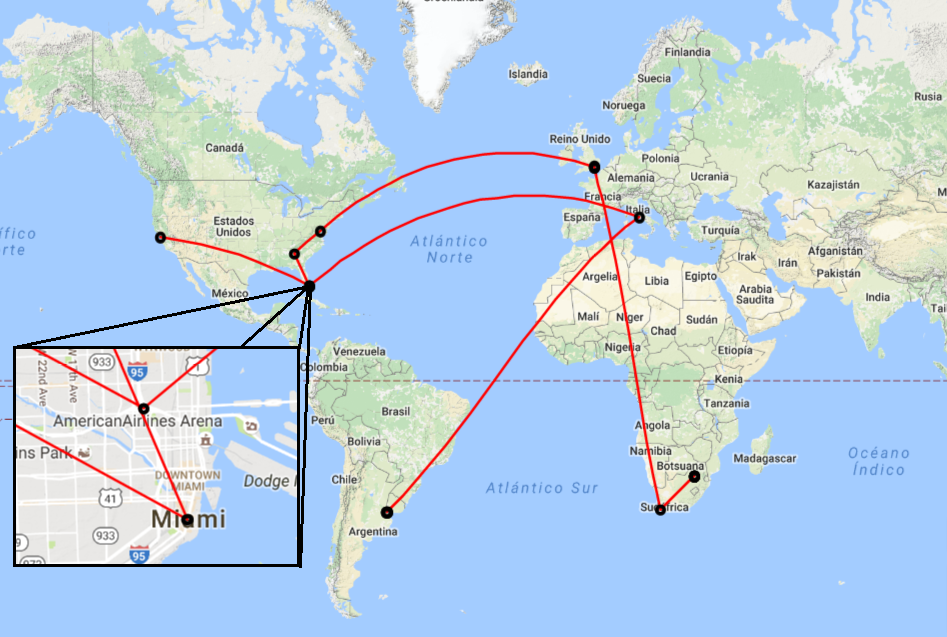
\includegraphics[scale=0.6]{imagenes/unisa-graficos/mapa-unisa.png}
  \caption{UNISA - Hops}
  \label{mapa-unisa}
\end{figure}

En este contexto, nos disponemos a realizar un análisis más profundo de nuestros resultados. Podemos observar entonces, que de los cuatro saltos intercontinentales, Cimbala identifica correctamente todos, salvo el de Argentina a Italia, y a su vez, indica 6 saltos como outliers que no son intercontinentales realmente. En resumen, si contamos todo outlier como salto intercontinental, obtenemos en esta muestra:

\begin{itemize}
	\item $26 \% $ de falsos positivos aprox.
	\item $4 \%$ de falsos negativos aprox.
	\item $70 \%$ de resultados acertados aprox.
\end{itemize}

Realizando un análisis parecido al de Oxford, en la figura \ref{fig:2} , podemos apreciar que la mayoría de los puntos se sitúan un poco por encima del 0.4 y cualquier otro punto que no respete esta línea, es considerado outlier( inclusive los valores de los ttls 20 y 22 están apenas por debajo, pero por debajo al fin y al cabo). Nuevamente observemos, que si nos quedamos solo con los puntos que se encuentran por encima de este valor, obtenemos exactamente los saltos intercontinentales, con excepción del de Argentina a Italia. Esto último probablemente se deba, a que, como se puede ver en la figura \ref{fig:1}, el ttl correspondiente a ese salto dá un rtt de 0.

\begin{figure}[!htbp]
  \centering
    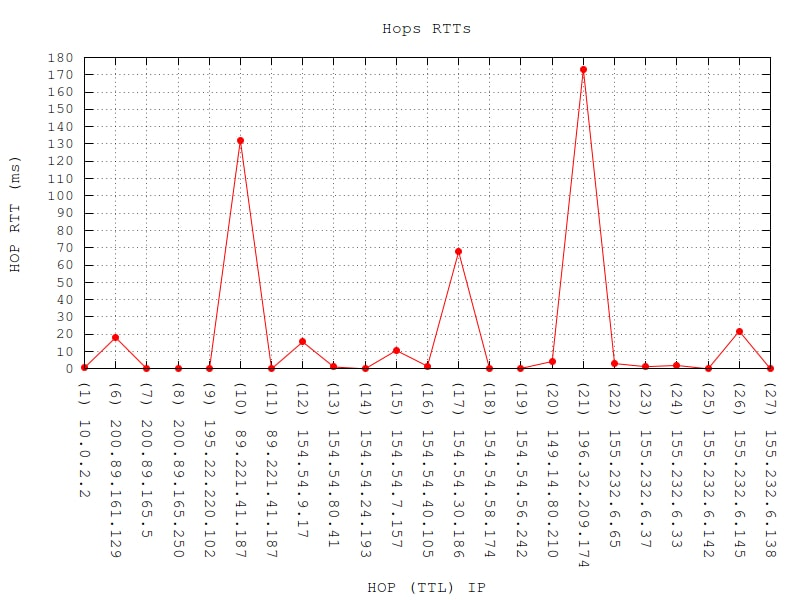
\includegraphics[scale=0.5]{imagenes/unisa-graficos/traceroute-unisa.jpg}
  \caption{UNISA- RTT hops}
  \label{fig:1}
\end{figure}


\begin{figure}[!htbp]
  \centering
    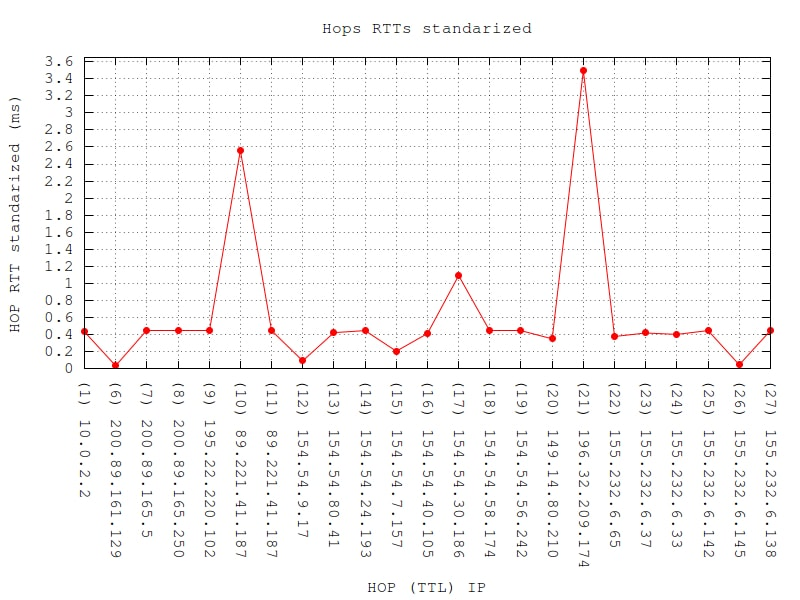
\includegraphics[scale=0.5]{imagenes/unisa-graficos/traceroute-unisa-standarized.jpg}
  \caption{UNISA- RTT hops standarized}
  \label{fig:2}
\end{figure}


Resumiendo, si consideramos solo los valores que en la figura \ref{fig:2} están por encima del punto de acumulaciónPONGANME UN BUEN NOMBRE, pasamos a obtener un $96\%$ de aciertos, siendo el $4\%$ restante un caso muy borde.



